%%%%%%%%%%%%%%%%%%%%%%%%%%%%%%%%%%%%%%%%%%%%%%%%%%%%%%%%%%%%%%%%%%%%%%%%%%%
%% This file is part of the book
%%
%% Algorithmic Graph Theory
%% http://code.google.com/p/graph-theory-algorithms-book/
%%
%% Copyright (C) 2009, 2010 Minh Van Nguyen <nguyenminh2@gmail.com>
%%
%% See the file COPYING for copying conditions.
%%%%%%%%%%%%%%%%%%%%%%%%%%%%%%%%%%%%%%%%%%%%%%%%%%%%%%%%%%%%%%%%%%%%%%%%%%%

\subfigure[$B_0$]{
\begin{tikzpicture}
[nodeDecorate/.style={shape=circle,inner sep=2pt,draw,thick}]
%% nodes or vertices
\node (1) at (0,0) [nodeDecorate] {};
%% stub nodes that should not be visible
\node () at (-0.5,0) [] {};
\node () at (0.5,0) [] {};
\end{tikzpicture}
}
%%
%%
\quad
\subfigure[$B_1$]{
\begin{tikzpicture}
[-,thick]
\node[shape=circle,inner sep=2pt,draw,thick] {}
  child {node[shape=circle,inner sep=2pt,draw,thick] {}};
%% stub nodes that should not be visible
\node () at (-0.5,0) [] {};
\node () at (0.5,0) [] {};
\end{tikzpicture}
}
%%
%%
\quad
\subfigure[$B_2$]{
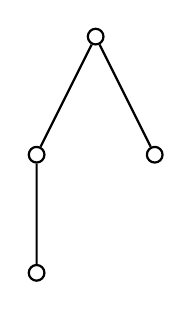
\begin{tikzpicture}
[-,thick,%
  every node/.style={shape=circle,inner sep=2pt,draw,thick}]
\node {}
  child {node {}
    child {node {}}
  }
  child {node {}};
\end{tikzpicture}
}
%%
%%
\quad
\subfigure[$B_3$]{
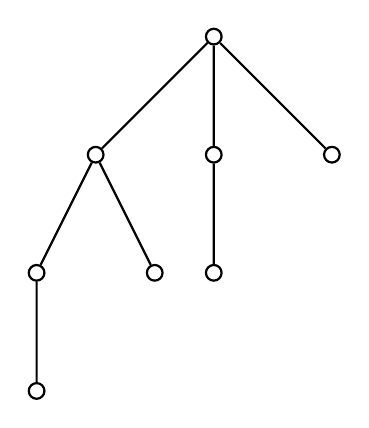
\begin{tikzpicture}
[-,thick,%
  every node/.style={shape=circle,inner sep=2pt,draw,thick}]
\node {}
  child {node {}
    child {node {}
      child {node {}}
    }
    child {node {}}
  }
  child {node {}
    child {node {}}
  }
  child {node {}};
\end{tikzpicture}
}
%%
%%
\subfigure[$B_4$]{
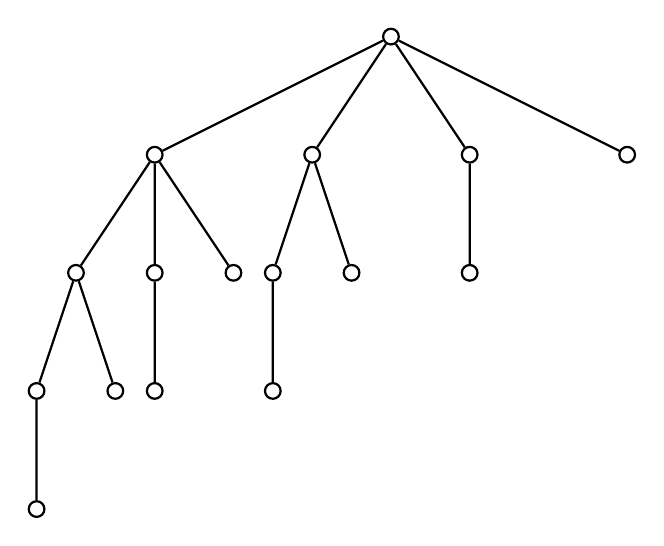
\begin{tikzpicture}
[-,thick,%
  every node/.style={shape=circle,inner sep=2pt,draw,thick}]
\node {}
  [sibling distance=2cm]
  child {node {}
    [sibling distance=1cm]
    child {node {}
      child {node {}
        child {node {}}
      }
      child {node {}}
    }
    child {node {}
      child {node {}}
    }
    child {node {}}
  }
  child {node {}
    [sibling distance=1cm]
    child {node {}
      child {node {}}
    }
    child {node {}}
  }
  child {node {}
    [sibling distance=1cm]
    child {node {}}
  }
  child {node {}};
\end{tikzpicture}
}
